% !TeX spellcheck = en_US
\section{Problem 5}

We are asked to generate an Auto Regressive (\textit{AR}) model and then create and RNN to predict it. 
Specifically, we chose to implement an LSTM as it has more parameters than GRU and is more adaptable to new information.

Samples must be generated from an AR model of the following form:
\[
X_t = 0.5 X_{t-1} - 0.1 X{t-2} + 0.2 X_{t-3} + U_t
\]
where $U_t$ is independent-identically distributed Uniform in the interval $\left( -0.25, 0.25 \right)$.

At first, we create the samples using \verb|generate_AR_data()| and the dataset for the neural network to train using \verb|create_dataset()|.

After creating all of the necessary data, we create a new model according to some predefined training sample sizes which are: $\left[100, 200, 500, 1000, 2000\right]$.
Calculation of valid loss and cost square error function is what follows the previous steps.

At the end, all cost functions are shown in figure~\ref{fig:prob5_mse}.

\begin{figure}[htpb]
	\centering
	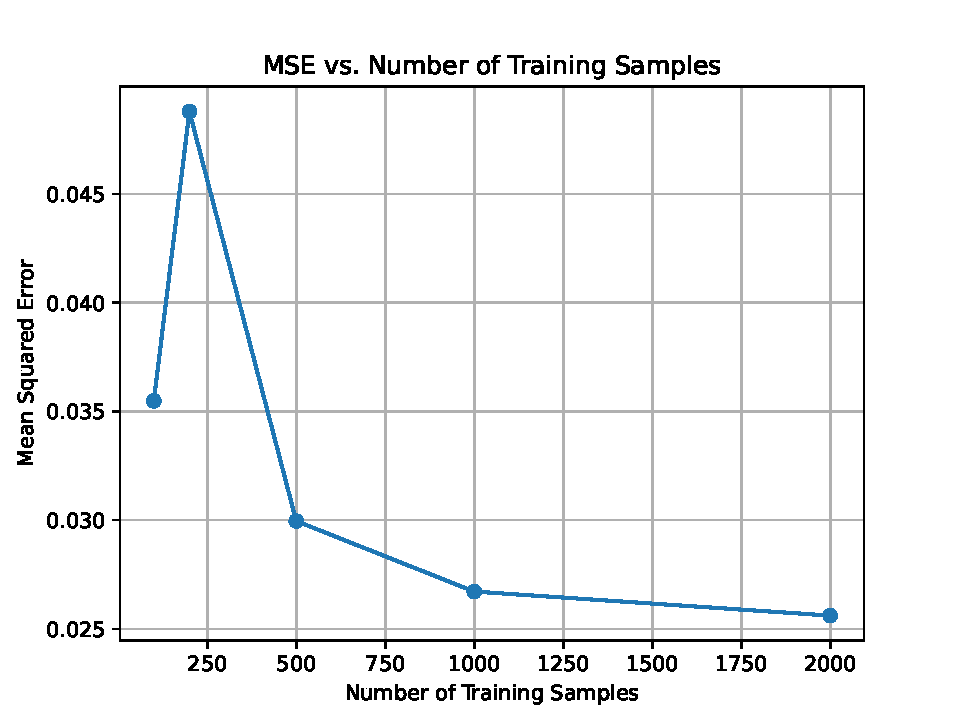
\includegraphics[width=0.5\linewidth]{../Problem 5/prob5_mse_vs_total_epoch.pdf}
	\caption{Averaged cost square error function over number of training samples}
	\label{fig:prob5_mse}
\end{figure}

The observed decrease in MSE with an increase in the number of training samples is indicative of the LSTM's capacity to learn and model the dependencies in the time series data. LSTMs are designed to capture long-term relationships, which is particularly advantageous for AR models where the future value is a function of past values.

The continuous improvement in prediction accuracy with more data suggests that the LSTM has not reached its capacity. Typically, there is a concern that a model may overfit to the training data if given too many examples; however, in this case, overfitting does not appear to be an issue. This could be due to the stochastic nature of the AR process and the noise term, which require the model to generalize well to perform accurately.

It's also worth noting the learning dynamics of LSTM networks. During the initial phase of training, the network rapidly learns the gross features of the time series. As training progresses, the rate of improvement in MSE slows down, suggesting that the model begins to refine its understanding of finer details within the data. This refinement process requires more nuanced examples, which can only be provided by larger datasets.